\subsection{Aprendizado de Máquina}

Segundo \citeonline{directions_ia_ml_dp}, o aprendizado de máquina é uma subcategoria da inteligência artificial que se refere à detecção de padrões importantes em uma base de dados. As ferramentas utilizadas aumentam a eficiência dos algoritmos no tratamento de grandes bases de dados.

Portanto, essa técnica permite que o computador melhore seus resultados com base na experiência, indicando uma relação direta entre a quantidade de dados consumidos pelo programa e a qualidade da solução do problema \cite{ml_explicado}.

Dentro desse nicho, existem outros subcampos, como: redes neurais, algoritmos evolucionários, algoritmos de busca, aprendizado por reforço, entre outros \cite{ml_oil_gas_industry}.

É possível observar uma hierarquia, ilustrada na \cref{fig:diagrama_ann}, entre o aprendizado de máquina e os principais termos, sendo eles: algoritmos de aprendizado de máquina que estão em um subconjunto chamado de aprendizado de máquina superficial, redes neurais artificiais que estão contidas no anterior e em um subconjunto chamado de aprendizado de máquina profundo, e redes neurais artificiais profundas que estão contidas em ambos os subconjuntos \cite{ml_and_dp}.

\begin{figure}[ht]
	\caption{Ilustração da relação entre os principais tópicos de aprendizado de máquina}
	\centering % para centralizarmos a figura
	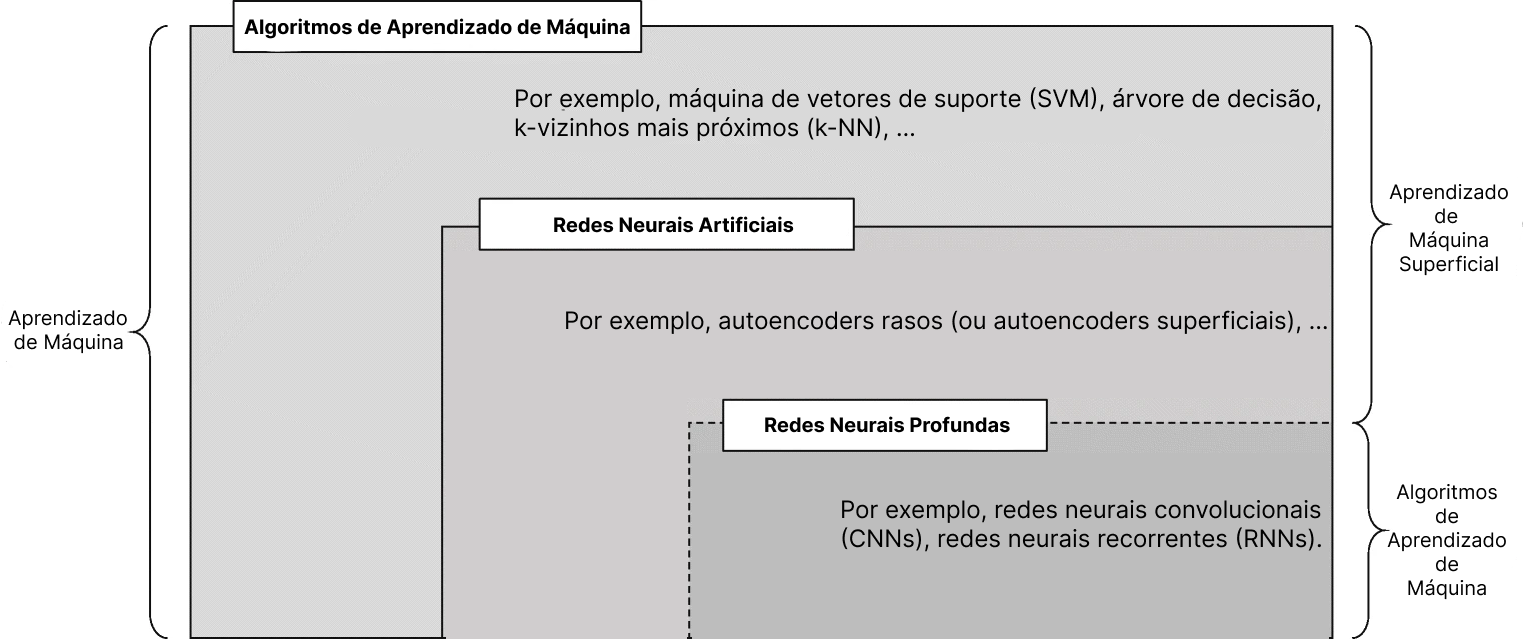
\includegraphics[width=10cm]{figures/diagrama_ann.png} % leia abaixo
	\legend{Fonte: \citeonline{ml_and_dp}}
	\label{fig:diagrama_ann}
\end{figure}
